\documentclass[twocolumn]{aastex631}
\usepackage{mathtools}
\usepackage{natbib}
\bibliographystyle{abbrvnat}
\setcitestyle{authoryear,open={(},close={)}}
\usepackage{txfonts}
\usepackage{lipsum, babel}
\usepackage[T1]{fontenc}
\usepackage{ae,aecompl}
\usepackage{xcolor,colortbl}
\usepackage{tikz}
\usepackage{graphicx}
\usepackage{url}
\usepackage{floatrow}
\usepackage{subfigure}
\usepackage{float}
\usepackage{amsmath}
\usepackage{amssymb}
\usepackage{cleveref}
\usepackage{physics}
\usepackage{empheq}
\usepackage{booktabs}
\usepackage{array}
\newcolumntype{R}[1]{>{\raggedleft\arraybackslash}p{#1}}
\newcolumntype{L}[1]{>{\raggedright\arraybackslash}p{#1}}
\usepackage{multirow}
\usepackage[flushleft]{threeparttable}
\usepackage{mathrsfs}
\usepackage{soul}
\pdfminorversion=5

\newcommand{\MyDiamond}[1][fill=black]{
\begin{tikzpicture}[x=1.2ex,y=1.2ex,line width=.1ex,line join=round, yshift=0.0ex]\
\draw  [#1]  (0,.5) -- (.5,1) -- (1,.5) -- (.5,0);
\end{tikzpicture}
}

\newcommand{\MyPlus}[1][fill=black]
{
\begin{tikzpicture}[x=1.5ex,y=1.5ex,line width=0.5ex]
\draw[#1] (0,.5) -- (1,.5);
\draw[#1] (.5,0) -- (.5,1);
\end{tikzpicture}
}

\newcommand{\MyCross}[1][fill=black]
{
\begin{tikzpicture}[x=1.ex,y=1.ex,line width=0.5ex]
\draw[#1] (0,0) -- (1,1);
\draw[#1] (0,1) -- (1,0);
\end{tikzpicture}
}

\newcommand{\MyTriangle}[1][fill=black]
{
\begin{tikzpicture}[x=1.ex,y=1.ex,line width=0.2ex]
\draw[#1] (0,1) -- (1,1);
\draw[#1] (1,1) -- (.5,0);
\draw[#1] (.5,0) -- (0,1);
\fill[#1] (0,1) -- (1,1) -- (.5,0) -- cycle;
\end{tikzpicture}
}

\newcommand{\MySolidLine}[1][fill=black]
{
\begin{tikzpicture}[x=2.ex,y=1.ex,line width=0.5ex]
\draw[#1] (0,.5) -- (2.5,.5);
\end{tikzpicture}
}

\newcommand{\MyDashedLine}[1][fill=black]
{
\begin{tikzpicture}[x=2.ex,y=1.ex,line width=0.5ex]
\draw [#1,dashed] (0,.5) -- (2.5,.5);
\end{tikzpicture}
}

\newcommand{\MyDashedDottedLine}[1][fill=black]
{
\begin{tikzpicture}[x=2.ex,y=1.ex,line width=0.5ex]
\draw [#1,dash dot] (0,.5) -- (2.5,.5);
\end{tikzpicture}
}

\newcommand{\MyDottedLine}[1][fill=black]
{
\begin{tikzpicture}[x=2.ex,y=1.ex,line width=0.5ex]
\draw [#1,dotted] (0,.5) -- (2.5,.5);
\end{tikzpicture}
}

\definecolor{Gray}{gray}{0.85}

\begin{document}
\title{The symmetry problem of the \textit{Fermi} and eROSITA bubbles: A proof-of-concept study}


\author[0000-0002-1868-0660]{Po-Hsun Tseng}
\affiliation{Institute of Astrophysics, National Taiwan University, Taipei 10617, Taiwan}

\author[0000-0003-3269-4660]{H.-Y. Karen Yang}
\affiliation{Institute of Astronomy, National Tsing Hua University, Hsinchu 30013, Taiwan}
\affiliation{Center for Informatics and Computation in Astronomy, National Tsing Hua University, Hsinchu 30013, Taiwan}
\affiliation{Physics Division, National Center for Theoretical Sciences, Taipei 10617, Taiwan}

\author[0000-0002-1249-279X]{Hsi-Yu Schive}
\affiliation{Institute of Astrophysics, National Taiwan University, Taipei 10617, Taiwan}
\affiliation{Department of Physics, National Taiwan University, Taipei 10617, Taiwan}
\affiliation{Center for Theoretical Physics, National Taiwan University, Taipei 10617, Taiwan}
\affiliation{Physics Division, National Center for Theoretical Sciences, Taipei 10617, Taiwan}

\author{Chun-Yen Chen}
\affiliation{Institute of physics, National Taiwan University, Taipei 10617, Taiwan}

\author[0000-0003-2654-8763]{Tzihong Chiueh}
\affiliation{Institute of Astrophysics, National Taiwan University, Taipei 10617, Taiwan}
\affiliation{Department of Physics, National Taiwan University, Taipei 10617, Taiwan}
\affiliation{Center for Theoretical Physics, National Taiwan University, Taipei 10617, Taiwan}


\correspondingauthor{Po-Hsun Tseng}
\email{zengbs@gmail.com}


\keywords{\textit{Fermi} bubbles, eROSITA bubbles, cosmic rays}

\begin{abstract}
The \textit{Fermi Gamma-Ray Space Telescope} reveals two large bubbles in the Galaxy,\
which extend nearly symmetrically $\sim50^{\circ}$ on either side of the Galactic center (GC).\
The recent discovery of giant eROSITA bubbles also shows a symmetrically enhanced X-ray\
emission from the shells around the eROSITA bubbles.\
To this end, previous simulation-based works based on active galactic nucleus (AGN) jets model\
assumed that the jets are vertical to the Galactic disk;\
however, there is a lack of preferred orientation of jets with respect to the Galactic disk.\
Using three-dimensional (3D) special relativistic hydrodynamic (SRHD) simulations that\
include cosmic rays (CRs) and thermal gas, we show that a thin interstellar medium (ISM) disk is an essential\
component for the symmetry \textit{Fermi} and eROSITA bubbles (collectively, Galactic bubbles).\
We also produce simulated gamma-ray and\
microwave spectra from the inverse Compton scattering and synchrotron,\
and compare them with the observed counterparts in order to verify\
an oblique AGN jets model. We find that\
(1) The simulated Galactic bubbles are nearly symmetric about the GC albeit\
the bipolar jets are at an angle $45^{\circ}$ with respect to\
the rotation axis of the Galatic plane (disc normal hereafter).\
(2) The edge of the eROSITA bubbles is a forward shock,\
originally driven by oblique bipolar jets emanating from the GC 12.39 million years ago,\
and significantly stretched by the stratified atmosphere afterwards.\
(3) Followed by the forward shock is a tangling contact discontinuity,\
which we interpret as the edge of the \textit{Fermi} bubbles\
composed of turbulent and high-temperature ($\sim2$ keV)\
plasma in pressure balance with the external medium.
(4) According to the microwave and leptonic gamma-ray spectra, the best-fitting\
CRe power-law index is found to be 2.4.\
The broad agreement between simulated and observed multiwavelength features\
has thus released a caveat:\
the jets shall be vertical to the disc normal.
\end{abstract}

\section{Introduction}
The detection of the \textit{Fermi} bubbles \citep{Su2012,Ackermann2014,Narayanan2017},\
two large bubbles symmetrically extending about 50 degrees above and below the Galactic plane,
is one of the great discoveries made with \textit{Fermi} Large Area Telescope \citep{Atwood2009}.

The gamma-ray emission of the \textit{Fermi} bubbles is observed in the energy range\
of 1--100 GeV and has an almost spatially uniform hard\
spectrum, sharp edges and an approximately flat brightness distribution.\

Over the course of a decade,\
the first all-sky X-ray survey with high-spatial resolution \citep{Predehl2021}\
from eROSITA \citep{Predehl2020} also reveals\
a giant hourglass-shaped structure (eROSITA bubbles hereafter) at the GC,\
extending about twice as large as the \textit{Fermi} bubbles.\
The large-scale X-ray structure\
shows that the intrinsic size of the bubbles is 14 kpc across \citep{Predehl2021},
and displays morphological symmetry about the Galactic plane as the \textit{Fermi} bubbles.

Their symmetry about the GC suggests that they originate\
from powerful energy injections from the GC, possibly related to nuclear star formation\
\citep{PhysRevLett.106.101102,Carretti2013}
or past AGN activity \citep{Guo2012,Yang2017}.

Early attempts \citep{Sarkar2015,Yang2017,Zhang2020}\
to model the symmetric Galactic bubbles\
assumed that the jets are vertical to the Galactic plane. However,\
observation \citep{Gallimore2006} has proposed that\
there is a lack of preferred orientation of jets with respect to the disc normal.\
In contrast, a number of galaxies in which the jets are oblique to the disc normal\
(e.g. NGC 3079, \citealt{Cecil2001}; NGC 1052, \citealt{Dopita2015}),\
including galaxies in which the jets lie in the plane of the disc (e.g. IC 5063, \citealt{Morganti2015}).

To this end, this work introduces a dense, thin disc of ISM\
around a jet source to deflects and decelerates the oblique jets,\
in an attempt to resolve the symmetry problem of the Galactic bubbles.\

The main purpose of this study is to use 3D\
special relativistic hydrodynamics simulations\
involving CR jet injections from the central SMBH in the Galaxy to investigate\
whether the \textit{oblique} jet scenario is able to produce\
the \textit{symmetric} Galactic bubbles that are\
consistent with the observed features, including the shape, the\
surface brightness, and the spectra of \textit{Fermi} bubbles \citep{Ackermann2014}\
and of microwave haze \citep{Dobler_2008,PlanckCollaborationIX2013}.

This paper is organized as follows.\
In Section \ref{Methodology}, we describe the numerical techniques and initial conditions employed.\
In Section \ref{Results}, we first present characteristics of our simulated Galactic bubbles,\
and then discuss how the disk affect the formation of the bubbles.\
We directly compare the morphology and profile of simulated eROSITA bubbles with\
observred X-ray map in Section \ref{X-ray},\
and also present the simulated and observed multiwavelength spectra of\
the \textit{Fermi} bubbles in Section \ref{sec:gamma-ray-microwave}.\
Finally, the summary and implications of our findings are given in Section \ref{Conclusions}.


\section{Methodology}
\label{Methodology}
  We used the GPU-accelerated special relativistic hydrodynamics AMR code (\textsc{gamer-sr}) developed at the\
  National Taiwan University\
  (Schive et al. \citeyear{gamer-1}, \citeyear{gamer-2}; \citeauthor{tseng2021} \citeyear{tseng2021})\
  to carry out the simulations of the Galactic bubbles by CR and relativistic fluid injections from the GC.

  As stressed by \citet{Yang2012}, CR diffusion has an insignificant effect\
  on the overall morphology of the \textit{Fermi} bubbles,\
  but only sharpens the edges of the simulated bubbles by the interplay between magnetic fields\
  and anisotropic CR diffusion with suppressed perpendicular diffusion across the bubble surface.

  Moreover, the magnetic fields within the \textit{Fermi} bubbles should be weak due to\
  adiabatic expansion, and thus the fields has\
  a little effect on the overall dynamics.

  For these two reasons,\
  we have ignored the CR diffusion and the magnetic field throughout\
  the simulation.\
  Also, we do not simulate the spectral evolution of the CR\
  and assume the pressure ratio of CR to gas is much less than 1 so that\
  the contribution of CR pressure gradient to the momentum of the gas can be ignored.\
  (we will see that the pressure ratio is around 0.1--0.2 throughtout the bubbles formation)\
  Over and above, we neglect the cooling and heating processes of CRs,\
  such as energy losses due to synchrotron and inverse Compton emission,\
  and CR reacceleration in shocks/turbulences.

  In this approach, we treat CRs as a single species without distinction between electrons and protons,\
  and directly evolve the CR energy density $e_{\text{cr}}$\
  as a function of $\mathbf{r}$ and $t$.\
  The CRs are advected with the thermal gas, and in return the velocities of gas\
  can react to the gradients of the CR pressure via the source term\
  containing spatial divergence of fluid velocities.


  Since the relativistic fluid ejected by the jet source\
  is quickly stalled off and slowed down by the dense ISM in a short time,\
  and the relativistic fluid\
  accounts for a little minority of total mass inside the simulation box,\
  we still use the Newtonian gravity to attack this problem.

  The governing equations solving the special relativistic ideal fluid\
  including CR advection, and dynamical coupling between the thermal gas and CRs without CR diffusion\
  can be written a succinct form as


  \begin{subequations}
    \label{governing-eq}
    \begin{align}
     &\partial_{t} D+\partial_{j} \left(DU^{j}/\gamma\right)=0,\label{D evolution}\\
     &\partial_{t} M^{i}+\partial_{j} \left(M^{i}U^{j}/\gamma+p_{\text{total}}\delta^{ij}\right)=\
     -\rho\partial_{i}\Phi,\label{M evolution}\\
     &\partial_{t} \tilde{E}+\partial_j \left[\left(\tilde{E}+p_{\text{gas}}\right)U^{j}/\gamma\right]=0, \label{E evoltion}\\
     &\partial_{t} \left(\gamma e_{\text{cr}}\right) + \partial_{j} \left(e_{\text{cr}}U^{j}\right)=\
     -p_{\text{cr}} \partial_{j} U^{j},\label{D evolution}
    \end{align}
  \end{subequations}


  where the five conserved quantities of gas $D$, $M^{i}$, and $\tilde{E}$ are the mass density,\
  the momentum densities, and the reduced energy density, respectively.\
  The reduced energy density is defined by subtracting the rest mass energy density of gas\
  from the total energy density of gas.\
  $\gamma$ and $U^{j}$ are the temporal and spatial component of four-velocity of gas.\
  $\rho$ is the gas density in the local rest frame defined by $D/\gamma$.\
  $p_{\text{gas}}$ is the gas pressure.\
  $p_{\text{cr}}$ and $e_{\text{cr}}$ are the CR pressure and CR energy density measured in the local rest frame.\
  $p_{\text{total}}$ is the sum of $p_{\text{gas}}$ and $p_{\text{cr}}$.\
  Note that we simply replace $p_{\text{total}}$ by $p_{\text{gas}}$ in this paper\
  as we have assumed $p_{\text{cr}}\ll p_{\text{gas}}$.\
  $\Phi$ is a gravitational potential.\
  $c$ is the speed of light, and $\delta^{ij}$ is the Kronecker delta notation.\
  Throughout this paper, Latin indices run from 1 to 3, except when stated otherwise.\

  The set of \Cref{governing-eq} is closed by using the Taub-Mathews equation of state \citep{Taub,TM_EOS}\
  that approximates the exact EoS \citep{Synge} for ultra-relativistically\
  hot gases coexisting with non-relativistically cold gases.

  \textsc{gamer-sr} adopts a new algorithm \citep{tseng2021} to convert between\
  primitive ($\rho$, $U^{j}$, $p$) and conserved variables ($D$, $M^{j}$, $\tilde{E}$),\
  significantly reducing numerical error caused by catastrophic cancellations\
  that commonly occur within the regions with high Mach number flows. e.g., jet-ISM interaction zones.

  \textsc{gamer-sr} also adaptively and locally reduce the min-mod coefficient\
  \citep{tseng2021} within the failed patch group rarely occurring in the SRHD solver,\
  new patches allocations, and ghost-zone interpolations.\
  In this manner, we provide an elegant approach to avoid the use of pressure/density floor,\
  being unnatural but widely used in almost publicly available codes.\

  \subsection{The Galactic and Disk Models}
  As a proof-of-concept study, we approximate conventionally axisymmetric stellar potential of Milky Way\
  by a plane-parallel potential that is symmetric about the mid-plane, or the Galactic plane, $z=0$\
  in a simulation box size of\
  $14\times14\times28$ kpc, slightly larger than the size of eROISTA bubbles.

  The plane-parallel potential is fixed throughout our simulations and given by
  \begin{equation}
    \Phi_{\text{total}}(z) = \Phi_{\text{bulge}}(z) + \Phi_{\text{halo}}(z),
  \end{equation}
  where
  \begin{equation}
    \Phi_{\text{bulge}}(z)=\
    2\sigma^2_{\text{bulge}}\
    \ln\cosh\left(z\sqrt{\frac{2\pi G\rho_{\text{bulge}}^{\text{peak}}}{\sigma^2_{\text{bulge}}}}\right)
  \end{equation}
  is the potential of an isothermal slab mainly contributed by stars around the Galactic bulge, and\
  $\Phi_{\text{halo}}(z)=v^2_{\text{halo}}\ln\left(z^2+d^2_{\text{h}}\right)$\
  is a plane-parallel dark logarithmic halo potential.

  With the help of the isothermal and hydrostatic equilibrium conditions,\
  and assuming the interfaces between the isothermal disc and atmosphere are in thermal pressure equilibrium,\
  we can write the steady-state gaseous density distribution,\
  confined in the total potential, of the disc and  Galactic atmosphere as\
  \begin{subequations}
  \begin{align}
     \displaystyle \rho_{\text{isoDisk}}(z) = \rho_{\text{isoDisk}}^{\text{peak}}
     \exp\left[-\frac{\Phi_{\text{total}}(z)}{k_{B}T_{\text{isoDisk}}/m_{\text{p}}}\right]&\label{isothermal-disc-density}\\
     \text{, if $|z| < z_{0}$,}& \nonumber \\
     \nonumber\\
     \displaystyle \rho_{\text{atmp}}(z) = \rho_{\text{atmp}}^{\text{peak}}
     \exp\left[-\frac{\Phi_{\text{total}}(z)}{k_{B}T_{\text{atmp}}/m_{\text{p}}}\right]&\label{isothermal-atmp-density}\\
     \text{, otherwise,}& \nonumber
  \end{align}
  \label{disc-atm-sys}
  \end{subequations}
  where $m_{\text{p}}$ is the proton mass,\
  $T_{\text{isoDisk}}$ and $T_{\text{atmp}}$ is the temperature of the isothermal disc and atmosphere,\
  $\rho_{\text{isoDisk}}^{\text{peak}}$ and $\rho_{\text{atmp}}^{\text{peak}}$ is the peak mass density\
  of the disc and atmosphere on the mid-plane $z=0$.

  We tabulate parameters in the first four\
  categories of \Cref{table-parameters},\
  except for $\rho_{\text{atmp}}^{\text{peak}}$ that\
  can be derived from the other known parameters and thermal pressure equilibrium condition\
  on the interfaces $(z=\pm z_{0})$ between the disc and atmosphere.\

  The density profile of \Cref{disc-atm-sys} is shown in \Cref{fig__initial-density-profile}.\
  Beyond the core radius ($\sim 2 \text{ kpc}$) the gaseous density decreases rapidly as a power-law.

%  The density profile of \Cref{disc-atm-sys} is shown in \Cref{fig__initial-density-profile}\
%  and compared to the observed result \citep{Miller_2013} beyond 1 kpc.\
%
%  Note that there is an difficulty in disentangling the contribution\
%  of the Local Bubble, a supernova remnant in which the Solar System is embedded \citep{Snowden1990},\
%  and the contribution from solar wind charge-exchange processes, which produce soft\
%  X-ray emission throughout the Solar System. As a result, the density profile of the Galactic halo remains unclear\
%  \citep{BlandHawthorn2016}.

  \begin{figure}
    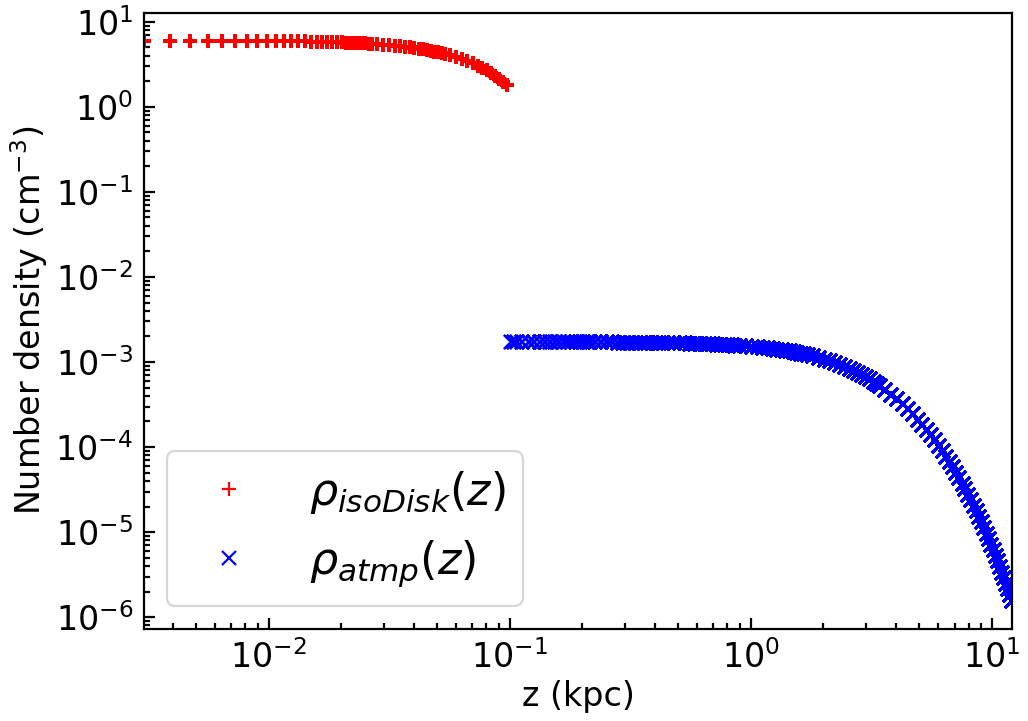
\includegraphics[width=\columnwidth]{figures/fig__initial-density-profile.png}
    \caption{The density profile of the isothermal disc (red pluses) and\
             atmosphere (blue crosses) along the positive z-axis.\
             The density distribution is derived from hydrostatic equilibrium,\
             the interface ($z=0.1$) between the isothermal disc\
             and the atmosphere is pressure balanced.}
    \label{fig__initial-density-profile}
  \end{figure}



  To quantify the synchrotron radiation as a function of position,\
  we adopt the default exponential magnetic field in \textsc{galprop} \citep{Strong2007}
  that obeys the following spatial dependence:\

  \begin{equation}
     |\mathbf{B}(R, z)|=B_{0}\exp\left[-\frac{z}{z_{0}}\right]\exp\left[-\frac{R}{R_{0}}\right],
     \label{magnetic-field}
  \end{equation}


  where $R=\sqrt{x^{2}+y^{2}}$, $B_{0}$ is the average field strength at the GC,\
  and $z_{0}$ and $R_{0}$ are the characteristic scales in the vertical and radial\
  directions, respectively. We adopt $z_{0} = 2$ kpc and $R_{0} = 10$ kpc, which\
  are best-fitting values in the \textsc{galprop} model to reproduce the\
  observed large-scale 408 MHz synchrotron radiation in the Galaxy.\
  We choose $B_{0} = 50$ $\mu$G based on the observed field strength at the\
  GC \citep{Crocker2010}.

   % The dispersion:
   %   2010-Comparing the statistics of interstellar turbulence in simulations and observations
   %   2011-RELATIVISTIC JET FEEDBACK IN EVOLVING GALAXIES


  \subsection{The Clumpy Multiphase Interstellar Medium}

  A crucial component in our work is the clumpy ISM disc initialized by\
  the publicly available pyFC code
  \footnote{\url{https://pypi.python.org/pypi/pyFC}}.\

  pyFC randomly generates dimensionless 3D scalar field $f(\bold{x})$\ % that is clumpy and porous.
  that obeys the log-normal probability distribution\
  with mean $\mu$ and dispersion $\sigma$,\
  and follows the power-law Kolmogorov spectrum
  \begin{equation}
    D(\bold{k})=\int k^{2} \hat{f}(\bold{k})\hat{f}^{*}(\bold{k})d\Omega \propto k^{-\beta},
    \label{Kolmogorov-spectrum}
  \end{equation}
  where $\hat{f}(\bold{k})$ is the Fourier transform of $f(\bold{x})$.\
  The spectrum $D(\bold{k})$ in the Fourier space is characterized by a power-law index $\beta=5/3$,\
  a Nyquist limit $k_{\text{max}}$, and a lower cutoff wave number $k_{\text{min}}$.
  $k_{\text{max}}$ is one-half of the spatial resolution within the disc,\
  and $k_{\text{min}}$ is 375.0, corresponding to the maximum size of an individual clump $\sim 20$ pc.\
  \citet{LA2002} and \citet{Wagner2012} have outlined a detailed procedure\
  for constructing a clumpy scalar field, and we do not repeat here.

  The density of the clumpy disc can thus be obtained by taking the scalar products of\
  $f(\bold{x})$ with $\rho_{\text{isoDisk}}(z)$ over all cells within the disc, i.e.,\
  $\displaystyle\rho_{\text{ismDisk}}(\bold{x}) =\
  f(\bold{x}) \rho_{\text{isoDisk}}(z)$.\
  Also, the thermal pressure equilibrium within the clumpy disc implies that the temperature of the disc is
  $\displaystyle T_{\text{ismDisk}}(\bold{x}) =\
  T_{\text{isoDisk}}(z)\rho_{\text{isoDisk}}(z)/\rho_{\text{ismDisk}}(\bold{x})$.


  The last category in \Cref{table-parameters} summarize the parameters of the clumpy disc and their references.

  On the basis of this setup, we cover the AMR base level with\
  $16\times16\times32$ root cells, refined progressively on the mid-plane $z=0$\
  based on the gradient of mass density.\
  We also restrict the refinement level at 7 within the disc so that\
  a molecular cloud can be adequately resolved by approximately 30 cells along their diameter, 20 pc.

  In this way, we plot the volume filling factor as a function of\
  initial number density within the disc without the jet source in \Cref{fig__numberDensityHistogram},\
  and show a close-up view of the\
  pressure, temperature, and number density slices
  in the y-z plane through the center of the disc in \Cref{fig__zoom-in-disc} .

  \begin{figure}
      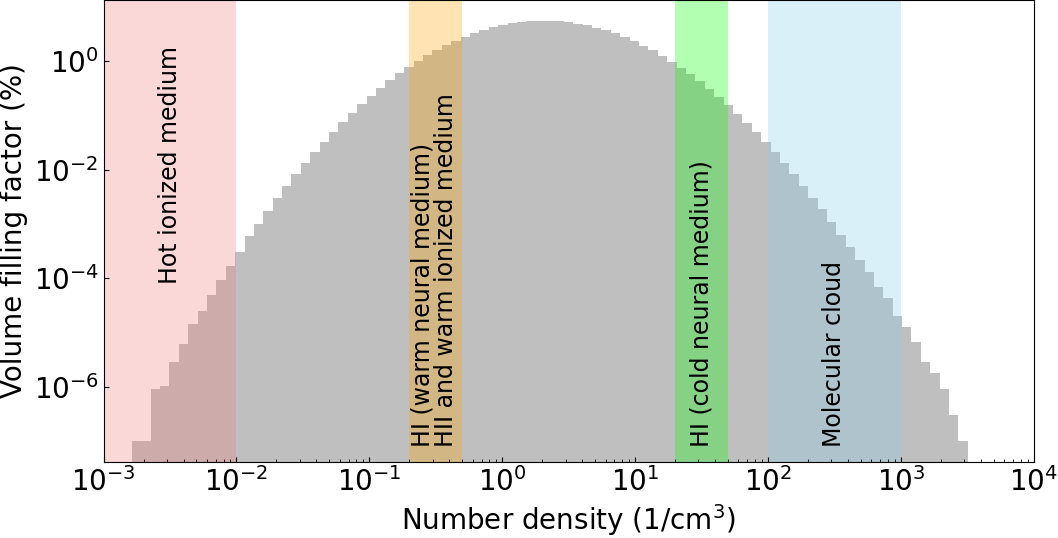
\includegraphics[width=\columnwidth]{figures/fig__numberDensityHistogram.png}
    \caption{The volume filling factor as a function of\
             initial number density within the disc without jet source.\
             The vertical bands from left to right depict the allowable number densities \citep{peak-ism-density} for\
             hot ionized, warm neutral (WNM), warm ionized (WIM), cold neutral mediums (CNM), and molecular clouds.}
      \label{fig__numberDensityHistogram}
  \end{figure}

  \begin{figure}
    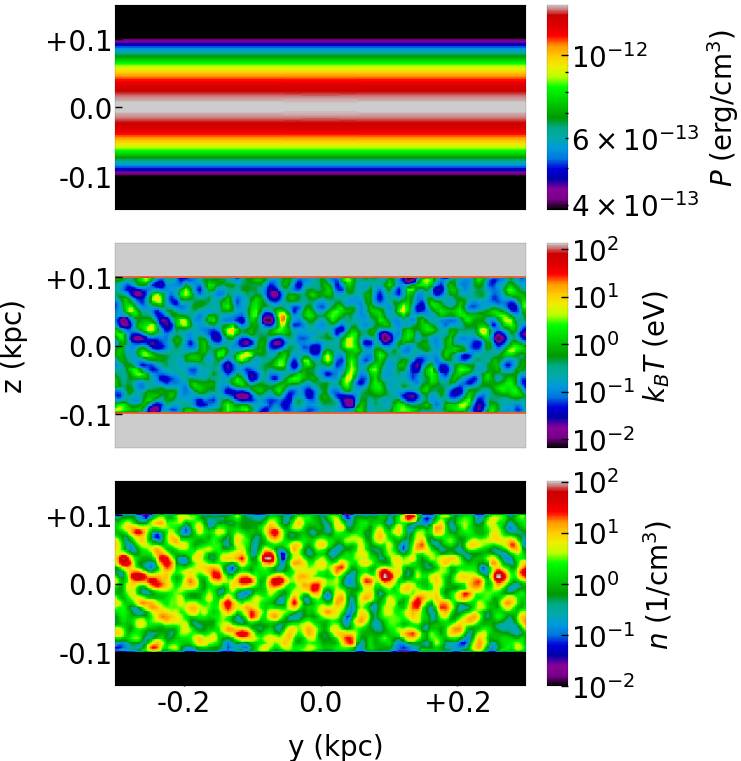
\includegraphics[width=\columnwidth]{figures/fig__zoom-in-disc.png}
    \caption{Close-up view of the initial\
             pressure (top), temperature (middle), and number density (bottom) slices\
             in the y-z plane through the center of the disc.
             }
    \label{fig__zoom-in-disc}
  \end{figure}

\begin{table*}[t]
\raggedright
\caption{Parameters of the disc, atmosphere, and gravitational potential in the simulations.}
\label{table-parameters}
\begin{tabular}{@{}llrc@{}}
\toprule[1pt]\midrule[0.3pt]
Parameter                             & Description                               & Value                                &  Reference                     \\ \midrule
{\bf Static stellar potential }       &                                           &                                      &                                \\
$\sigma_{\text{bulge}}$               & Velocity dispersion of bulge              & 100 km$\cdot$s$^{-1}$                & \citep{velocity-dispersion-MW} \\
$\rho_{\text{bulge}}^{\text{peak}}$   & Peak average density of bulge             & $4\times 10^{-24}$ g$\cdot$cm$^{-3}$ &   N/A                          \\ \hline
{\bf Static dark halo potential }     &                                           &                                      &                                \\
$v_{\text{halo}}$                     & Characteristic velocity                   & 131.5 km$\cdot$s$^{-1}$              & \citep{Johnston1995}           \\
$d_{\text{h}}$                        & Core radius                               & 12 kpc                               & \multicolumn{1}{c}{''}         \\ \hline
{\bf Atmosphere }                     &                                           &                                      &                                \\
$T_{\text{\text{atmp}}}$              & Temperature of atmosphere                 & $10^{6}$ K                           & \citep{temperature-MW}         \\ \hline
{\bf Isothermal disc }                &                                           &                                      &                                \\
$z_{0}$                               & Scale height of disc                      & 100 pc                               & \citep{peak-ism-density}       \\
$T_{\text{\text{isoDisk}}}$           & Temperature of disc                       & $10^{3}$ K                           & \multicolumn{1}{c}{''}         \\
$\rho_{\text{isoDisk}}^{\text{peak}}$ & Peak mass density of disc                 & $10^{-23}$ g$\cdot$cm$^{-3}$         & \multicolumn{1}{c}{''}         \\ \hline
{\bf Clumpy disc }                    &                                           &                                      &                                \\
$\dagger$  $k_{\text{min}}$           & Cutoff wave number                        & 375.0                                & \citep{peak-ism-density}       \\
$\mu$                                 & Mean of scalar field                      & 1.0                                  &   N/A                          \\
$\ddag$  $\sigma$                     & Dispersion of scalar field                & 5.0                                  & \citep{Federrath2010}          \\
$\beta$                               & Power law index                           & -5/3                                 &   N/A                          \\ \midrule
\end{tabular}
\begin{tablenotes}
      \raggedright
      \item  $\dagger$  $k_{\text{min}}=375.0$ leads to the size of an individual molecular cloud $\sim 100$ pc.
      \item  $\ddag$ In numerical simulations of turbulence,\
             \citet{Federrath2010} find $\sigma\sim 3.6$ and 35 for solenoidal (divergence-free)\
             and compressive (curl-free) driving force,\
             respectively, so that our adopted value of 5 is closer to their solenoidal result.
    \end{tablenotes}
\end{table*}


% In addition to the gravitational interaction, we ignore other interactions between stars and gases.
% We also ignore the self-gravity of the ISM disc and of the atmosphere.
% We ignore the centrifugal force of Milky Way rotation acting on the bubbles.
%

\subsection{Inclined jet injection}

  We simulate the jet with an inclination angle\
  $45^{\circ}$ with respect to the Galactic plane\
  in order to release the caveat that\
  the jet direction must be perpendicular to the Galactic plane, and in particular to\
  investigate how the dense disc affect the bubbles formation.


  A few additional quantities are used to characterize the jets:
  the density contrast between the thermal gas contained in the jet source and the atmosphere gas,\
  $\rho_{\text{jet}}/\rho_{\text{amb}}=10^{-3}$,\
  the temperature contrast, $T_{\text{jet}}/T_{\text{amb}}=2\times10^{4}$,\
  the pressure ratio of CR to gas is 0.18,\
  and the flow 4-velocity inside the jet source $\beta\gamma = 0.6$\
  along the symmetric axis of cylinder.\
  The jet power is thus $3.2\times 10^{42}$ erg/s, resulting in the Eddington ratio 0.008.

  Note that as we inject the jets at the center of the clumpy disc,\
  we define the atmosphere gas density by the peak density of\
  the isothermal disc on the mid-plane $z=0$ (i.e. $\rho^{\text{peak}}_{\text{isoDisk}}$),\
  as opposed to the \textit{clumpy} density around the jet source, to avoid ambiguous definition.


  The bipolar jets are constantly ejected from a cylindrical source at the beginning of simulation ($t=0$)\
  and suddenly quenched at $t=1.2$ Myr before fully breaking out the disc.\
  Without quenching, the Galactic bubbles at the present time will be asymmetric about the Galactic plane.
  The jet duration allows the total ejected energy to be $1.2\times10^{56}$ erg between\
  $8\times10^{55}$ erg and $1.3\times10^{56}$ erg, estimated by \citet{Predehl2020}.\



  The diameter and height of cylindrical source are 4 pc,\
  leading to the source volume ($\sim 50 \text{ pc}^{3}$) is\
  much smaller than that of an individual clump by a factor of about 83.\
  By intentionally reducing the volume ratio of the jet source to an individual clump,\
  we can mitigate the effect of the randomness of the clumps on the bubbles.\
  Moreover, we resolve the jet source with the highest refinement level 11,\
  bringing the finest spatial resolution up to 0.4 pc.\



\section{Results}
\label{Results}

\subsection{Morphology and properties of Galactic bubbles}

 \Cref{fig__jetI5+ismSeed3-45deg} shows\
 the slices of pressure (top), temperature (middle), number density (bottom)\
 at the end of simulation $t=12.39$ Myr.\
 The slices pass through the bipolar jet source injecting along $z=-y$ direction.

 The fiducial run (leftmost column) with the initial condition specified in Section \ref{Methodology}\
 shows that the edge of the outermost bubbles is indeed a forward shock,\
 expanding 12.5 kpc above and below the Galactic plane,\
 with a semiminor axis about 6.8 kpc on the plane.\
 We note that the overall extent of the outermost bubbles is comparable to\
 the two spherical objects of a radius 6-7 kpc proposed by \citet{Predehl2020} for modeling the eROSITA bubbles\
 based on X-ray emissions.

 The temperature profile (left middle panel in \Cref{fig__profile}) along the positive z-axis in\
 \Cref{fig__jetI5+ismSeed3-45deg} indicates that\
 the smooth region (purple band) emitting X-ray\
 is around 0.3-0.5 keV, similar to that observed by \citet{Miller2016} and \citet{Kataoka2018}.

 Followed by the forward shock is a turbulent and hot plasma.\
 As shown in the temperature or density slices of the fiducial run,\
 the full extent of the turbulent plasma is approximately agree with\
 that of the \textit{Fermi} bubbles \citep{Su2010}.
 Also, the temperature of the plasma is as high as 2 keV, comparable to few keV inside the \textit{Fermi} bubbles\
 obtained by observing X-ray absorption lines through the hot\
 gaseous halo along many different sight lines in the sky \citep{Miller_2013}.\
 We also note that the turbulence within the hot plasma is in pressure balance with the external medium,\
 suggesting the outer edge of the \textit{Fermi} bubbles\
 is a tangling contact discontinuity rather than a smooth shock \citep{Zhang2020}.

 The most interesting finding is that there is a innermost bubbles\
 (dashed box in left top panel of \Cref{fig__jetI5+ismSeed3-45deg})\
 extending out from the GC on either side of the thin disk.\
 The innermost bubbles are cold (1-10 eV), dense ($10^{-4}$--$10^{-2}$ cm$^{-3}$),\
 and underpressured with respect to the turbulent plasma.\
 Moreover, the close-up view (right column in \Cref{fig__profile}) of profiles\
 demonstrates that there is a sharp pressure jump and dense shell at $z=3.61$ kpc,\
 indicating that the innermost bubbles are an expanding reverse shock.\
 We also find that the turbulent plasma is bracketed between the downstream of reverse shock\
 and of the outermost forward shock, thus heating the turbulent plasma up considerably.

 We stressed that either the outermost, turbulent plasma, or innermost bubbles\
 are symmetric about the Galactic plane despite the jet is tilted to the disk normal\
 at an angle $45^{\circ}$.

 To explore how the disk affect the formation of the Galactic bubbles,\
 we compare the fiducial run (first column from left in \Cref{fig__jetI5+ismSeed3-45deg})\
 with the case adopting the smooth disc\
 (second column; \Cref{fig__initial-density-profile} shows the density profile) in a stratified atmosphere.\
 The results show that the initial density distribution of the dense disc has an insignificant effect\
 on the overall dynamics of bubbles. However, the outermost bubbles arising from the smooth disc\
 in an uniform atmosphere (third column) is spherical-shape,\
 suggesting the stratification facilitates the outermost bubbles elongation significantly.\
 Also, the two rightmost columns reveal that the development of the innermost bubbles\
 is always associated with the disc, without the disc,\
 the outermost bubbles and the turbulent plasma will be oblique,\
 indicating the dense disc is crucial for\
 the symmetry of the Galactic bubbles and for the innermost bubbles formation.


  \begin{figure}
    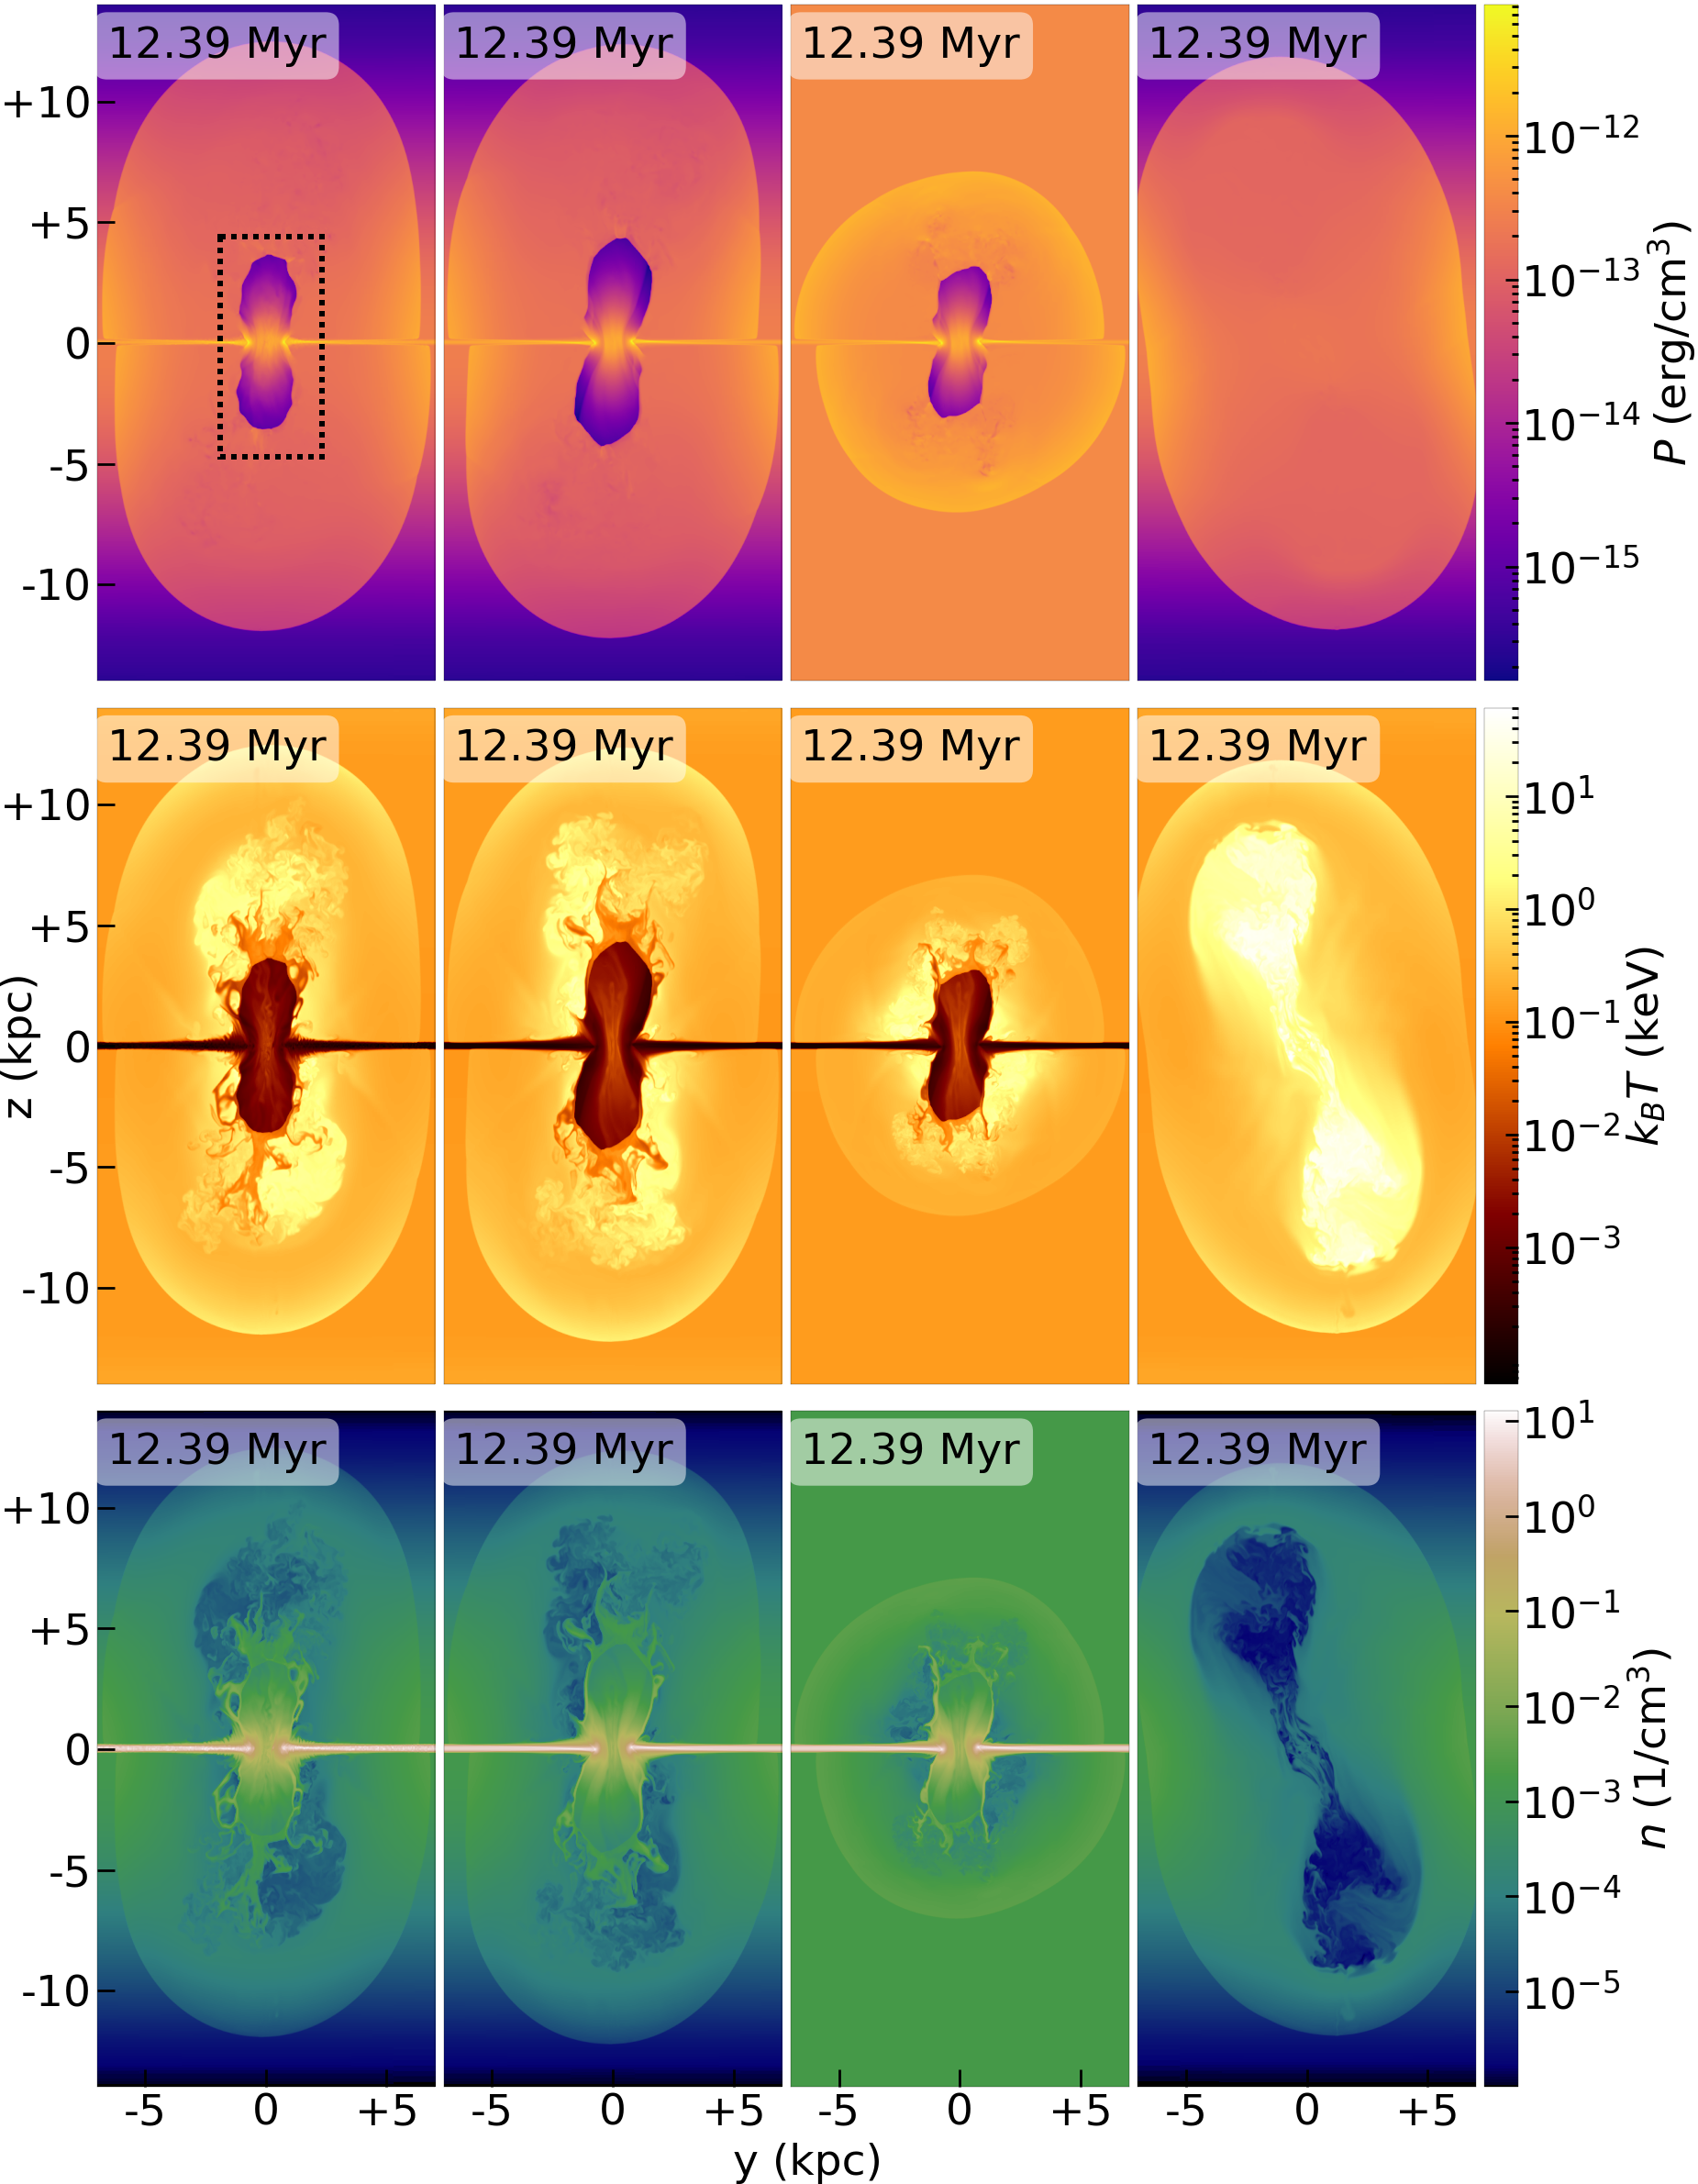
\includegraphics[width=\columnwidth]{figures/fig__jetI5+ismSeed3-45deg.png}
    \caption{
             The slices of pressure (top), temperature (middle), and number density (bottom)\
             at the end of simulation $t=12.39$ Myr.\
             The slices pass through a bipolar jet source injecting along $z=-y$ direction\
             for a duration $t=0$--$1.2$ Myr.\
             Comparison between the clumpy (first column from left)\
             and the smooth disc (second) in a stratified atmosphere\
             shows that the initial density distribution of the dense disc has an insignificant effect\
             on the overall dynamics of bubbles. However, the outermost bubbles arising from the smooth disc\
             in an uniform atmosphere (third) is spherical-shape,\
             suggesting the stratification facilitates the outermost bubbles elongation significantly.\
             Also, the two rightmost columns reveal that the development of the innermost bubbles\
             (dashed box in top left panel)\
             is always associated with the disc, without the disc,\
             the outermost bubbles and the turbulent plasma will be oblique,
             indicating the dense disc is crucial for\
             the symmetry of the Galactic bubbles and for the innermost bubbles formation.
             }
    \label{fig__jetI5+ismSeed3-45deg}
  \end{figure}

  \begin{figure}
    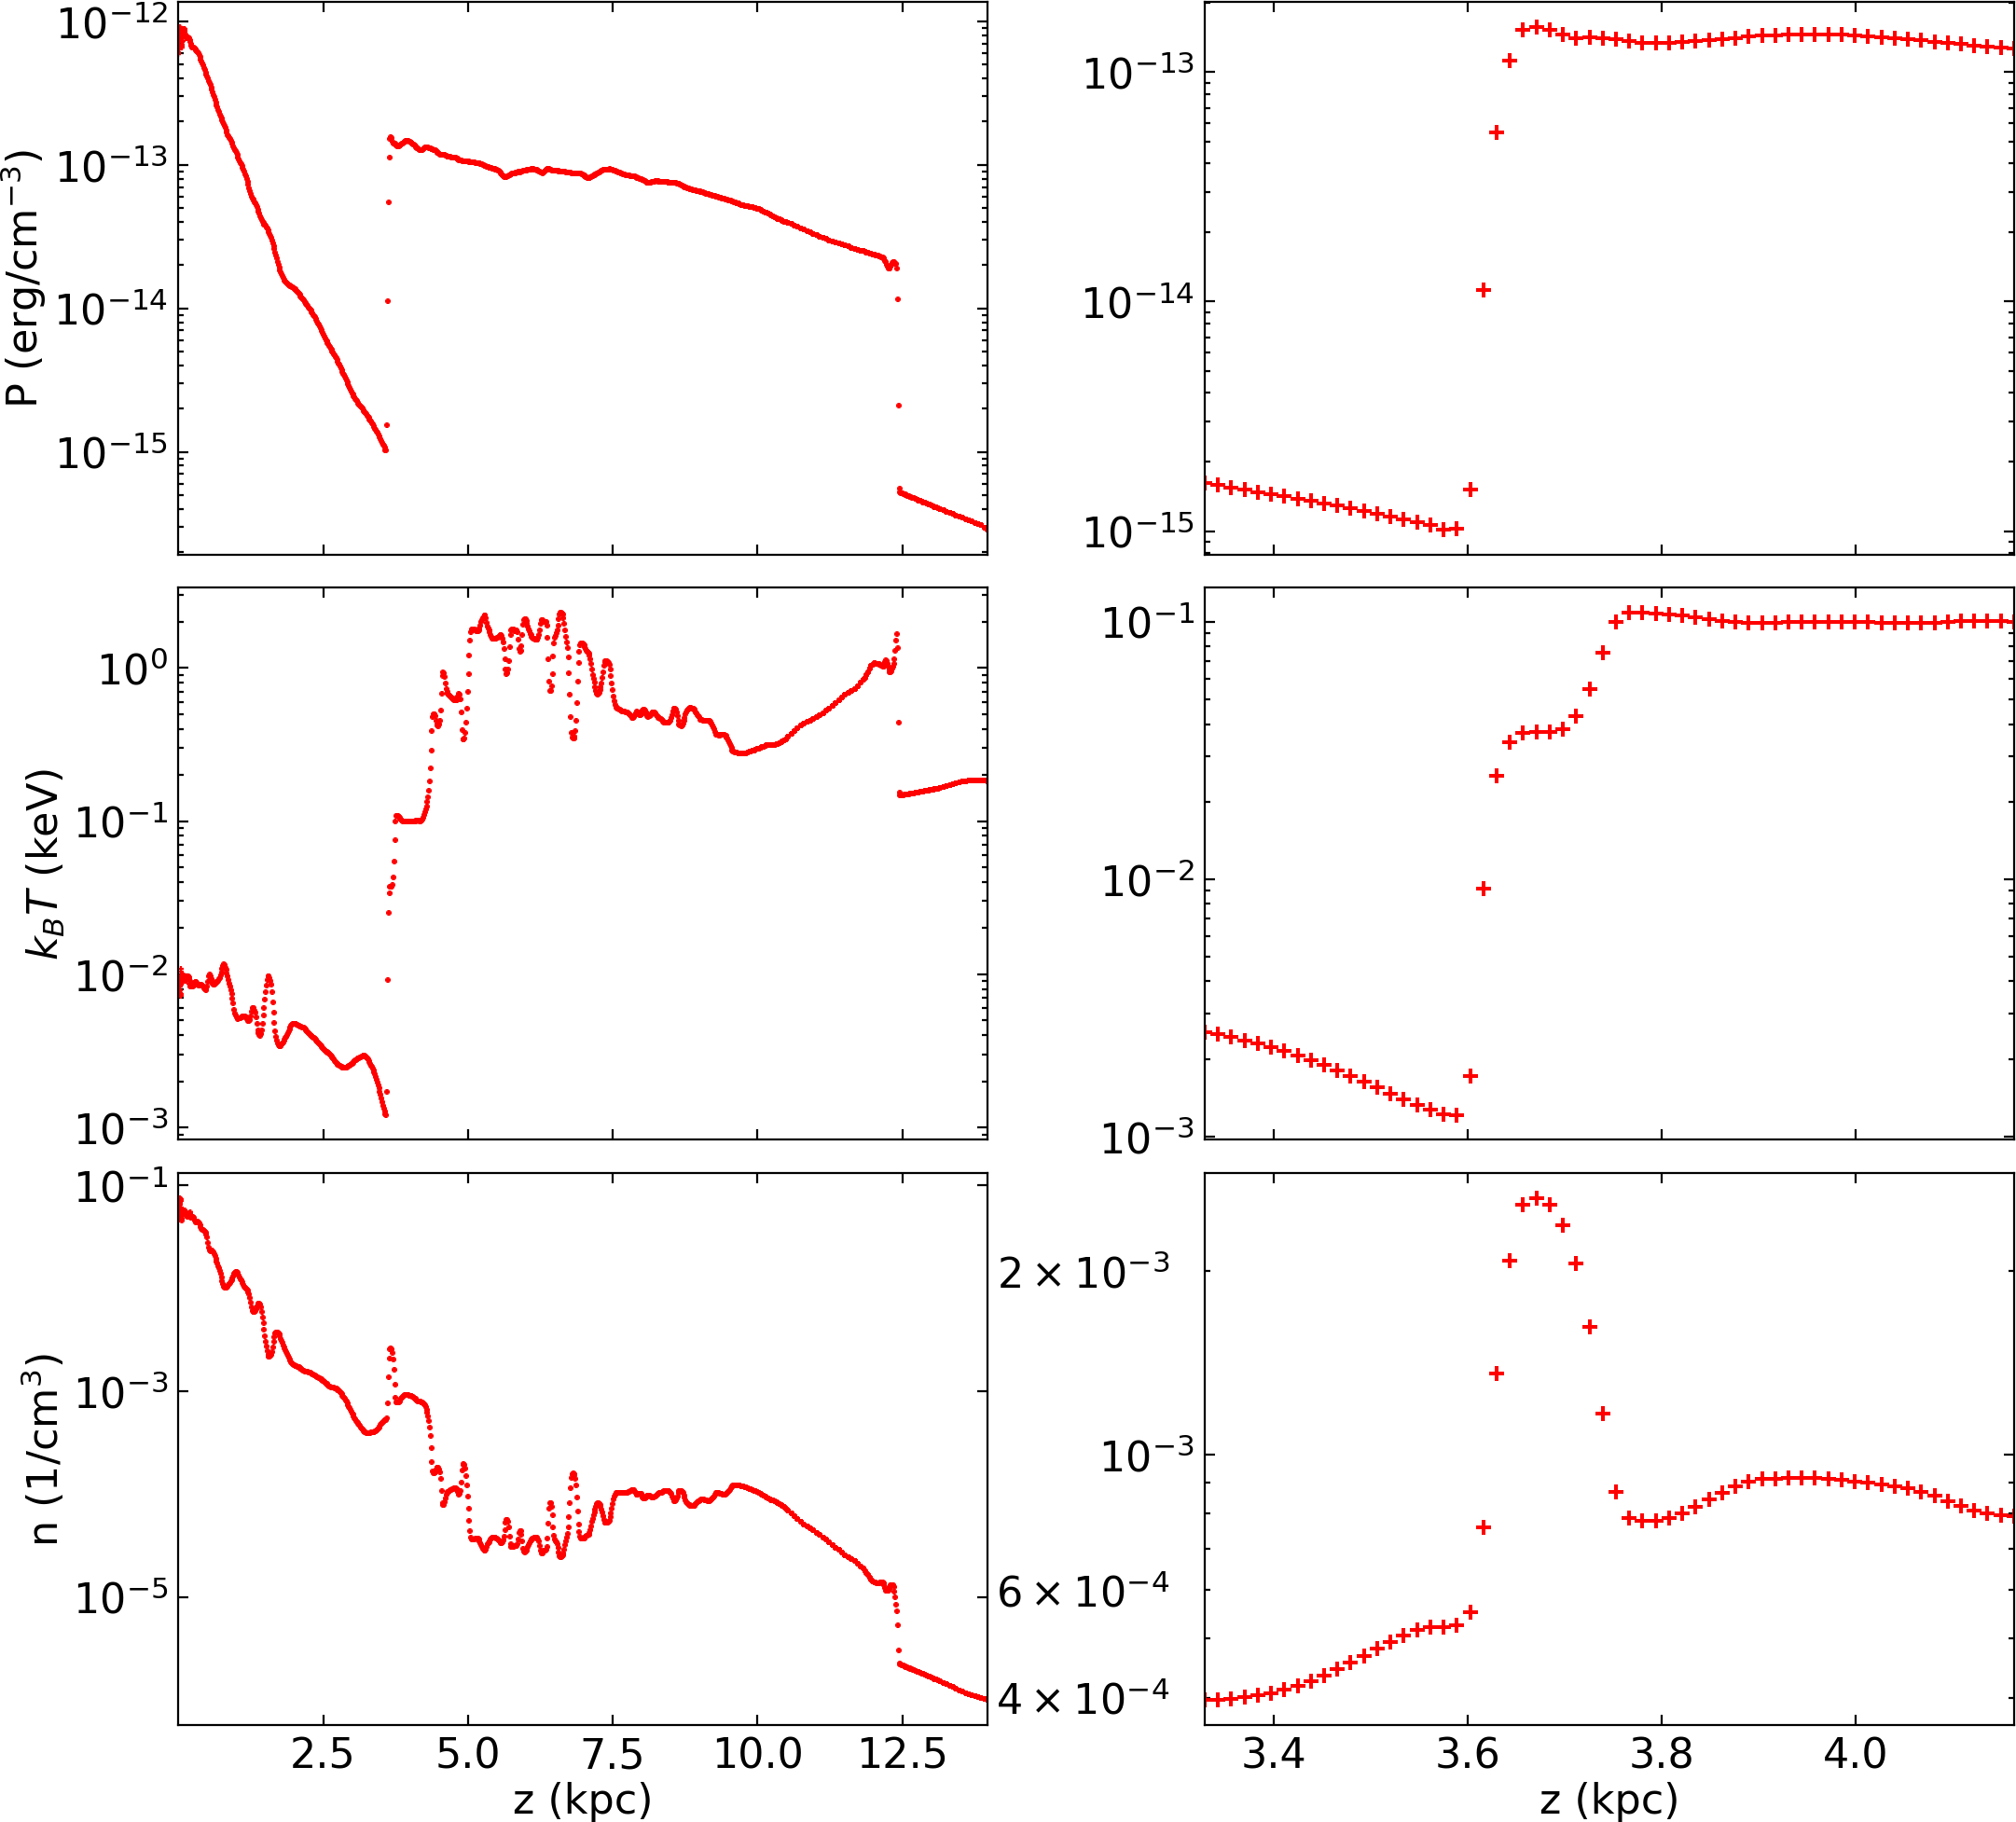
\includegraphics[width=\columnwidth]{figures/fig__profile.png}
    \caption{
             Left: the profiles of pressure (top), temperature (middle),\
             and number density (bottom)\
             along the positive z-axis in \Cref{fig__jetI5+ismSeed3-45deg}.
             Right: the close-up view of profiles in the yellow band.\
             The sharp pressure jump and dense shell at $z=3.61$ kpc\
             indicate that the innermost bubbles\
             (dashed box in top left panel of \Cref{fig__jetI5+ismSeed3-45deg})\
             are an expanding reverse shock.\
     }
    \label{fig__profile}
  \end{figure}

  \subsection{X-ray}
  \label{X-ray}
  The X-ray emissivity is computed\
  for each computational volume cell
  using the MEKAL model \citep{Xray-1,Xray-2,Xray-3}\
  implemented in the utility XSPEC \citep{XSPEC}, assuming solar metallicity.\
  The X-ray intensity map are then generated by projecting the emissivities\
  along lines of sight\
  pointing away from the solar position at $(R_{\odot},0,0)=(8,0,0)$ kpc\
  with angular resolutions of 0.5 degrees, where $R_{\odot}$ is the Sun-GC distance.

  We point out that the projections throughout this paper is \lq perspective\rq,\
  which has the effect of making distant object appear smaller than the same object in the near distance,\
  in order to facilitate a reliable interpretation of simulated all-sky map,\
  and also that the observed X-ray emission is contributed by all the gas in the Milky Way halo,\
  which likely extends to a radius of $\sim$250 kpc \citep{halo-radius-1,halo-radius-2},\
  much bigger than our simulation box.

  We first compute the X-ray emissivity\
  from the simulated gas within a radius of 25 kpc away from the GC.
  Then, beyond 25 kpc the gas is assumed to be isothermal with $T=10^6$ K and\
  follows out to a radius of 250 kpc the observed density profile of \citep{temperature-MW}.

  \Cref{fig__xray_0.8keV_angle_000} shows\
  the comparison between simulated (top) and observed (bottom) all-sky map\
  in the range 0.6--1.0 keV at 12.39 Myr and the present time, respectively.\
  In the simulated map, the red arrow at the center of map represents the direction of the bipolar jet,\
  constantly ejecting at an angle of $45^{\circ}$ to the disc normal between 0--1.2 Myr.

  \Cref{fig__x-ray-profile-0.8keV-000} displays the simulated count rate profiles (red)\
  in the same energy band as \Cref{fig__xray_0.8keV_angle_000}\
  cut at various galactic latitudes (as labelled), compared with the observation (black).\
  \Cref{fig_xray-map} is quite revealing in several ways.\

  First, we observe that\
  The simulated eROSITA bubbles are not as limb-brightened as the observation.\
  A possibility to enhance the X-ray emission is to include shock-accelerated CRs near the shock,\
  in which CRs could increase the compressibility of the fluid,\
  resulting in the enhanced thermal Bremsstrahlung emissivity that is proportional to density.
  The broad agreement between simulated and observed X-ray maps hints that\
  the full vertical extent of the eROSITA bubbles can be properly formed by an oblique jet within a thin disk\
  of dense ISM.

  Second, as shown in \Cref{fig__jetI5+ismSeed3-45deg},\
  the half-width of the outermost bubbles is around 7 kpc,\
  corresponding to an half angular width $\sin^{-1}(7 \text{ kpc}/R_{\odot})\sim122^{\circ}$,\
  which is as wide as the eROSITA bubbles in the simulated X-ray map (top panel in \Cref{fig__xray_0.8keV_angle_000}).\
  We therefore suggest that the eROSITA bubble shells are a signature of compressed forward shocks\
  that have been driven into the northern and the southern Galactic halo,
  as previously proposed by \citet{Predehl2020}.


% 2. North Polar Spur is not shown as it is a supernova remanent near us.
  Third, the innermost bubbles\
  shown in \Cref{fig__jetI5+ismSeed3-45deg},\
  even though with high column density, is invisible in the simulated X-ray map as\
  the temperature of innermost bubbles is around $1$--$10$ eV\
  (see the temperature profile in \Cref{fig__profile}).\
  Consequently, the X-ray emission within the innermost bubbles
  is severely suppressed by the cutoff $\exp\left[-h\nu/k_{B}T\right]$ in the thermal Bremsstrahlung emissivity.\
  This is the reason why the innermost bubbles is unseen in the observation.


  \begin{figure*}
    \subfigure[Simulated (top) and observed (bottom; \citealt{Predehl2020}) count rate\
               (photons s$^{-1}$ deg$^{-2}$) in the 0.6--1.0 keV range.\
               Throughout this paper we show sky maps\
               in Galactic coordinates centered on the Galactic center using a Hammer-Aitoff projection,\
               and observed from the solar system.\
               The red arrow at the center of the\
               top panel depicts the direction of the bipolar jet, constantly ejecting at an angle of $45^{\circ}$\
               to the disc normal in 1.2 Myr.]
     {
      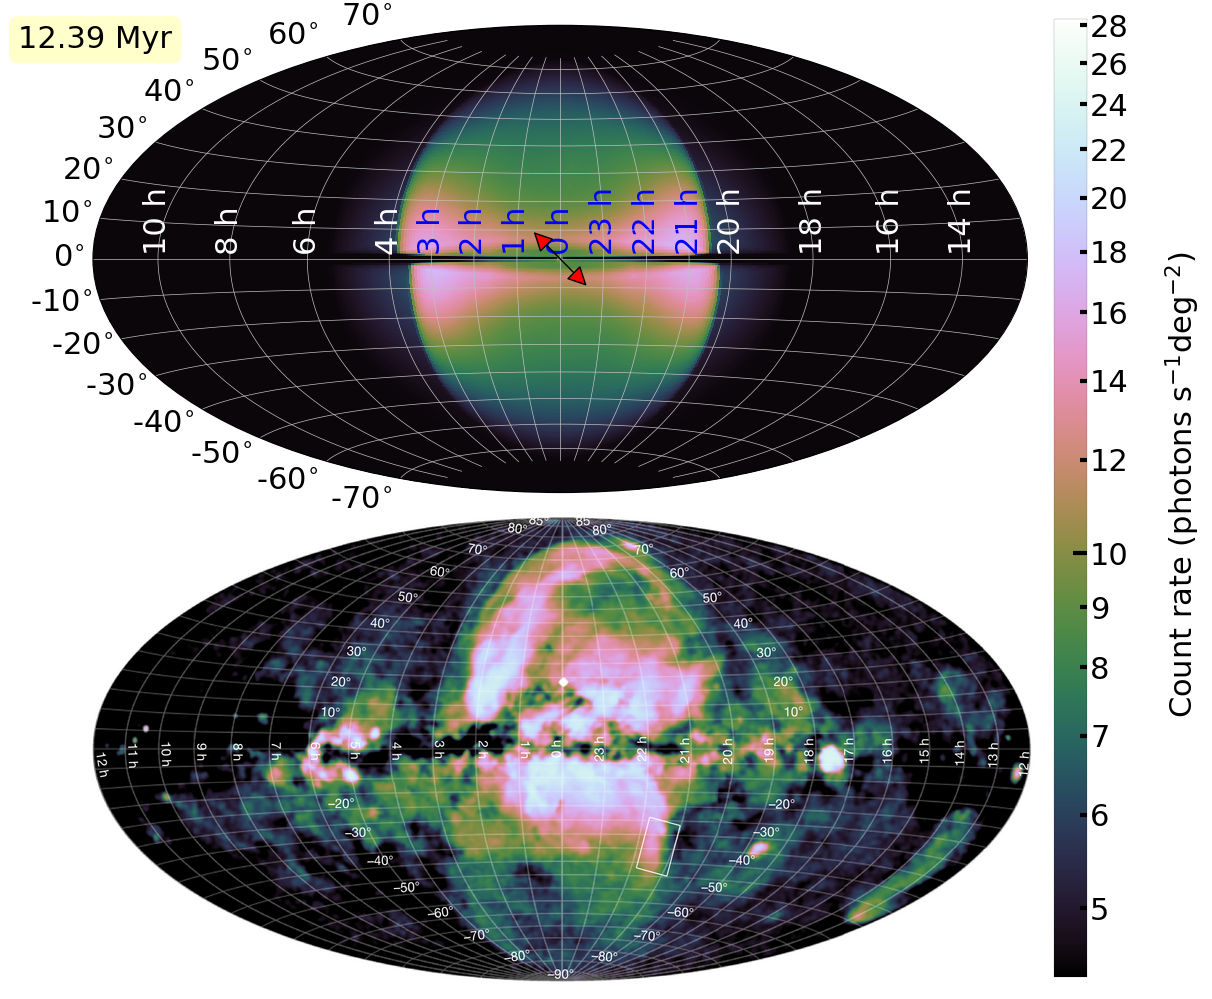
\includegraphics[width=0.8\linewidth]{figures/fig__xraymap.png}
      \label{fig__xray_0.8keV_angle_000}
     }
    \subfigure[Comparison of simulated (red) and observed (black; \citealt{Predehl2020}) one-dimensional\
               count rate profiles in the same energy band as \Cref{fig__xray_0.8keV_angle_000},\
               cut at various galactic latitudes (as labelled).]
     {
      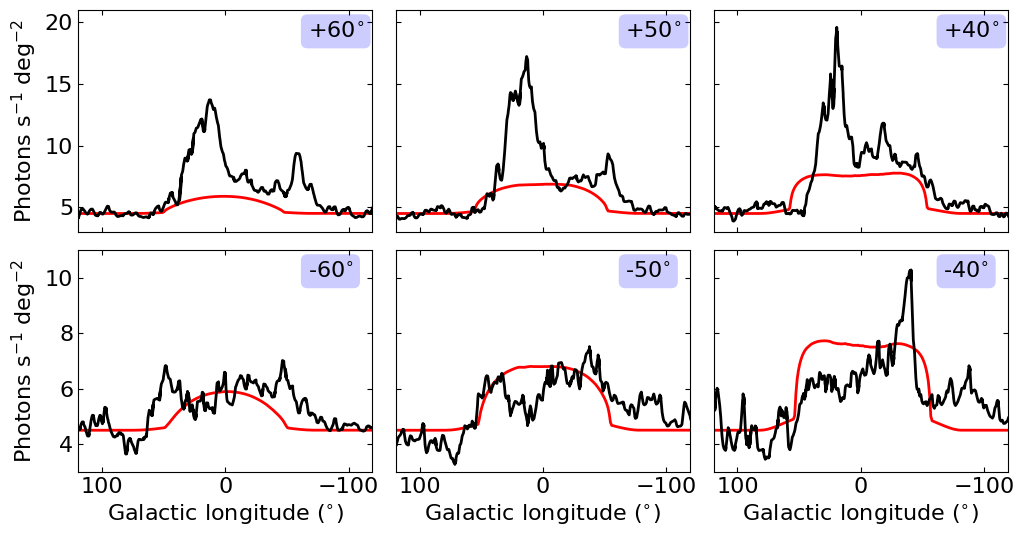
\includegraphics[width=0.8\linewidth]{figures/fig__xray-profile-0.8keV-000.png}
      \label{fig__x-ray-profile-0.8keV-000}
     }
    \caption{}
    \label{fig_xray-map}
  \end{figure*}



\subsection{Gamma-ray and microwave spectra: constraint on the CRe spectral index}
\label{sec:gamma-ray-microwave}
In this section, we give the constraint on the CRe spectral index by\
comparing the simulated gamma-ray and microwave spectra\
with the observed spectra of the Fermi bubbles \citep{Ackermann2014}\
and the microwave haze \citep{Dobler_2008}, respectively.\

The simulated gamma-ray and microwave spectra is based on the\
IC scattering and synchrotron from CRe, respectively, in which\
the CRe spectrum follows a power-law distribution ranging from\
$0.5$ MeV to $562.1$ GeV.

%The microwave haze at 23 GHz was first detected by the \textit{WMAP} \citep{Dobler_2008}\
%within the region $|b|<30^{\circ}$ above and below the Galactic plane,\
%and later confirmed by the Planck Collaboration IX \citep{PlanckCollaborationIX2013}.

The IC emissivity of the upscattered photons at the energy $\epsilon_{1}$ is computed for\
each computational cell in our simulations\
using the Klein-Nishina IC cross-section \citep{Jones1968,BLUMENTHAL1970}\
to handle the scattering between ultra-relativistic CRe and photons in the ISRF:

\begin{subequations}
  \begin{align}
  &\frac{dE}{dtd\epsilon_{1}dV} =\nonumber\\
               &\frac{3}{4}\sigma_{T}c\mathbb{C}\epsilon_{1}\int^{\epsilon_{\text{max}}}_{\epsilon_{\text{min}}}
               \frac{n(\epsilon)}{\epsilon}d\epsilon\int^{\gamma_{\text{max}}}_{\gamma_{\text{min}}\left(\epsilon\right)}
               \gamma^{-(p+2)}f(q, \Gamma)d\gamma,\\
  \nonumber\\
  &f(q, \Gamma) =\nonumber\\
               &2q\ln q+(1+2q)(1-q)+0.5(1-q)\frac{\left(\Gamma q\right)^2}{1+\Gamma q},\\
  &q=\frac{\epsilon_{1}/\gamma\
               m_{\text{e}}c^{2}}{\Gamma\left(1-\epsilon_{1}/\gamma m_{\text{e}}c^{2}\right)},\\
  &\Gamma=\frac{4\epsilon \gamma}{m_{\text{e}}c^2},\\
  &\gamma_{\text{min}}(\epsilon)=\
   0.5\left(\frac{\epsilon_{1}}{m_{\text{e}}c^2}+\sqrt{\left(\frac{\epsilon_{1}}{m_{\text{e}}c^2}\right)^2+\
   \frac{\epsilon_{1}}{\epsilon}}\right) \label{gamma-min},
  \end{align}
\label{gammaray-emissivity}
\end{subequations}

where $\sigma_{T}$ is the Thomson cross section, $c$ speed of light,\
$m_{\text{e}}$ electron mass,\
$n(\epsilon)$ the energy distribution of the photon number density in ISRF given by \citet{Porter2017},\
$\gamma$ the Lorentz factor of CRe,\
$\mathbb{C}$ and $p$ are the normalization constant and spectral index of CRe power-law spectrum.
$\gamma_{\text{min}}(\epsilon)$ is the minimum Lorentz factor of CRe\
that allows incident photons to scatter from energy $\epsilon$ to $\epsilon_{1}$.
$\gamma_{\text{max}}$ is the maximum CRe Lorentz factor in the spectrum.

We perform the double integration in \Cref{gammaray-emissivity} on each cell\
over the range of CRe Lorentz factor, and\
the range of incident photon energy between\
$\epsilon_{\text{min}}=1.13\times10^{-4}$ eV (cosmic microwave background) and\
$\epsilon_{\text{max}}=13.59$ eV (optical starlight)\
to obtain the simulated IC emissivities.


The synchrotron emissivity with an isotropic electron pitch angle distribution\
is given by \citet{BLUMENTHAL1970}:

\begin{subequations}
   \begin{align}
      &\frac{dE}{dtd\nu dV} =\nonumber\\
      &\frac{4\pi\mathbb{C}e^{3}B^{0.5(p+1)}}{m_{\text{e}}c^{2}}\
      \left(\frac{3e}{4\pi m_{\text{e}}c}\right)^{0.5(p-1)}\
      a(p)\nu^{-0.5(p-1)},\\
      &a(p)=\nonumber\\
           &\frac{2^{0.5(p-1)}\sqrt{3}\Gamma\left[\left(3p-1\right)/12\right]\
                                      \Gamma\left[\left(3p+9\right)/12\right]\
                                      \Gamma\left[\left(p+5\right)/4\right]}
      {8\sqrt{\pi}(p+1)\Gamma\left[\left(p+7\right)/4\right]},
   \end{align}
   \label{synchrotron-emissivity}
\end{subequations}

where $\Gamma$ is gamma function, $B$ is the magnetic field strength defined in\
\Cref{magnetic-field}.

For a given longitude and latitude range, the simulated spectra are\
computed by projecting emissivities\
as we project X-ray emissivities in Section \ref{X-ray},\
and then we average the spectra over all the sight lines within the region on sky.


\Cref{fig__gammaRaySynchtronSpectrum} shows the simulated microwave (left)\
and gamma-ray (right) spectra averaged over the different patches (shown in the legends) of the sky.\
The row from top to bottom shows the spectra with different CRe spectral index $2.2, 2.4$ and $2.6$.\
Several points are worth specific comment.\

First, we find that the simulated gamma-ray spectra are well fitted by\
the CRe spectral index 2.4 (the middle row),\
despite the simulated microwave spectra are marginally consistent with the observed.

Second, the simulated and observed gamma-ray spectra is\
nearly latitude independent, and characterized by a broad bump that roughly peaks around $\sim10$ GeV.\
However, the high-latitude spectrum tends to be slightly dimmer than low-latitude\
probably because the optical intensity in ISRF decays with increasing latitude.

Third, the gamma-ray spectra for all latitudes indicate a spectral cutoff around energies 400--500 GeV,\
remarkably consistent with the observed cutoff energy.\
This is expected since\
the upscattered high-energy photons ($\epsilon_{1}\sim450$ GeV) mainly arise from\
the scatterings between the relativistic CRe ($\gtrapprox 408$ GeV)\
and optical starlight ($\epsilon \sim 10$ eV).\
Thus, \Cref{gamma-min} can be reduced to $\epsilon_{1}\sim\gamma m_{\text{e}}c^2$\
in the Klein--Nishina limit\
$\left(\text{i.e. }\epsilon_{1}\epsilon \gg \left(m_{\text{e}}c^2\right)^2\right)$,\
implying most of the CRe energy is carried away by the upscattered photons.

Fourth, the good agreement between the simulated and observed gamma-ray/microwave spectra\
imply that, in the presence of ISRF and magnetic fields, the emission of the Fermi bubbles and\
the microwave haze can be produced by the same high-energy electrons\
via inverse Compton scatterings and synchrotron radiations, respectively,\
as previously suggested \citep{Su2010,Dobler2012}.

\begin{figure*}
  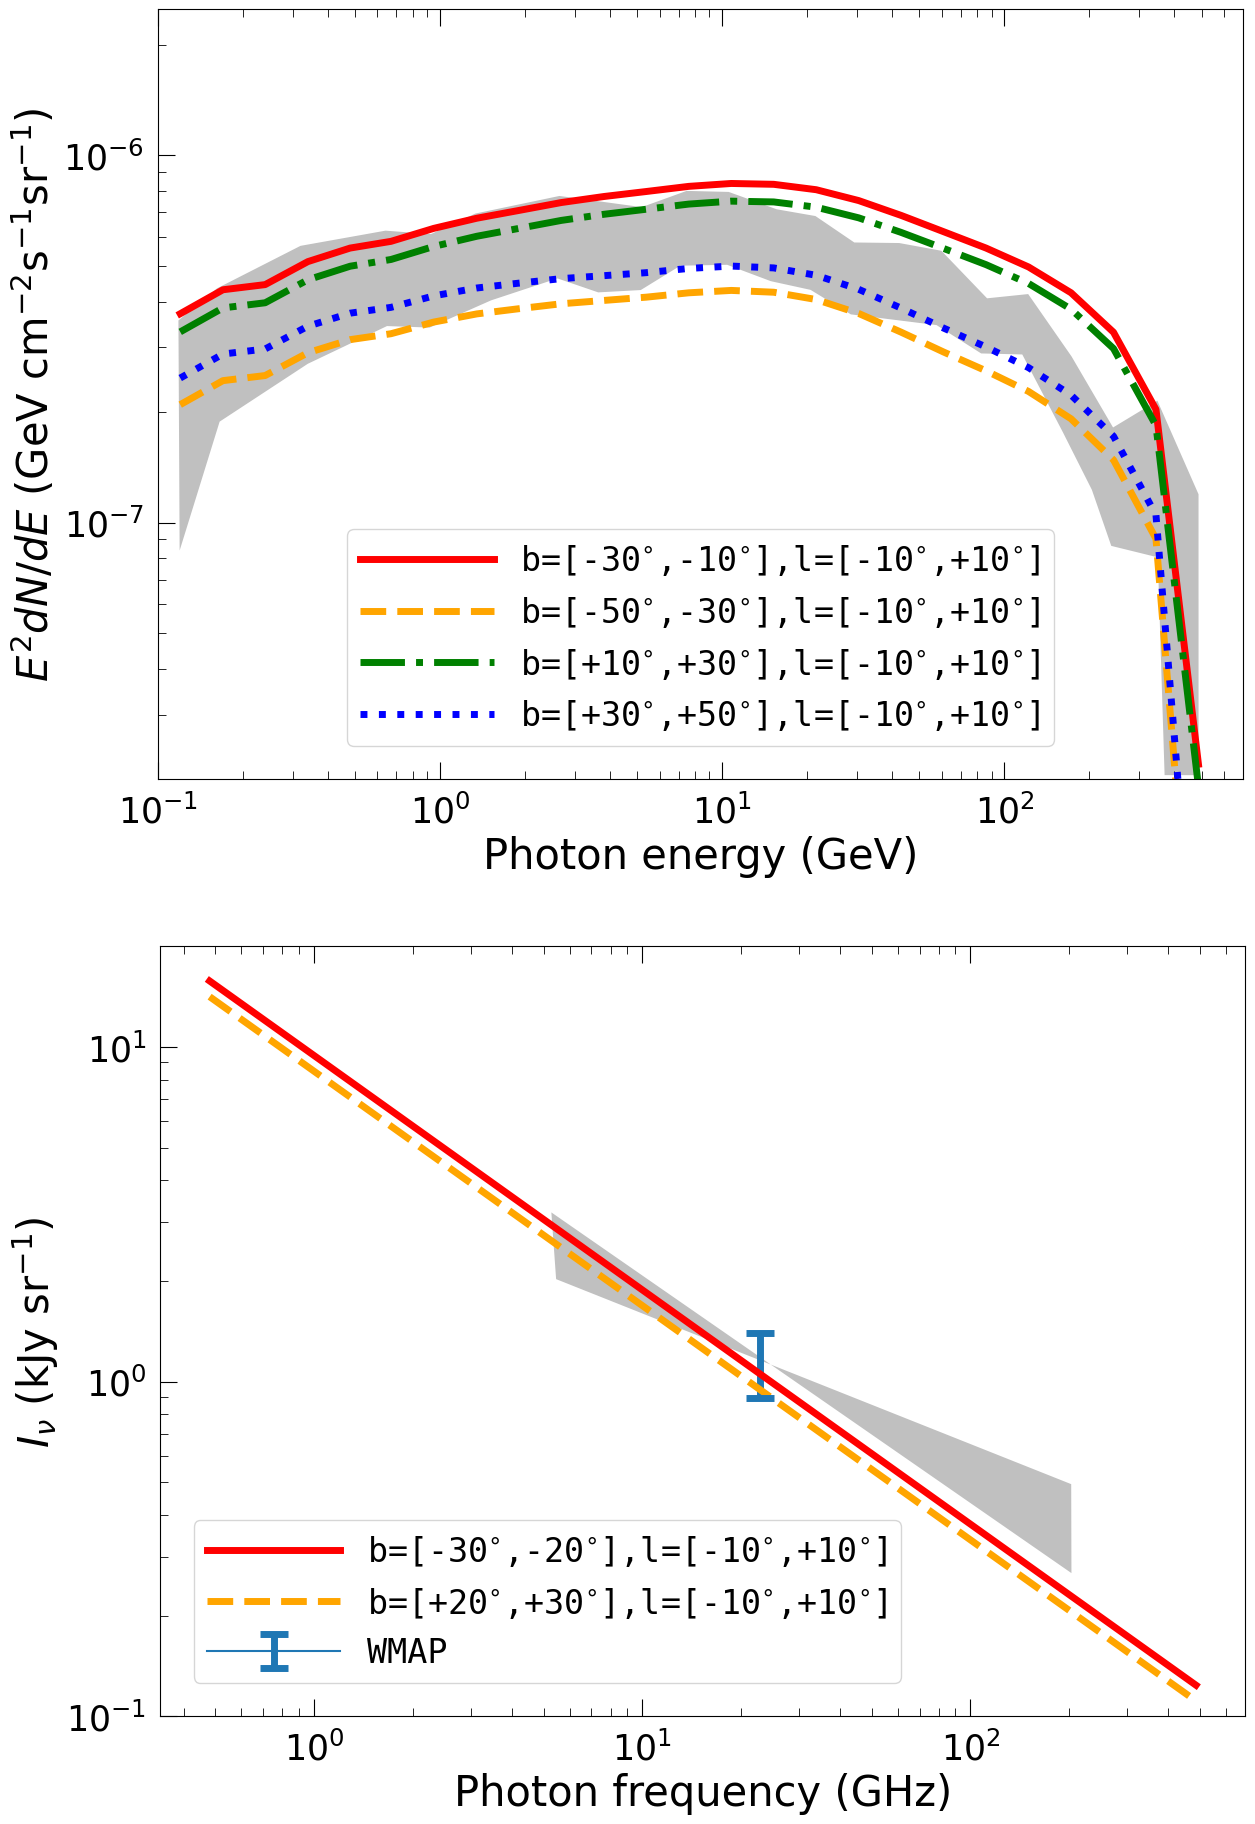
\includegraphics[width=\linewidth]{figures/fig__spectrum.png}
  \caption{
      Simulated microwave spectra (colored lines in left) averaged over $20^{\circ}<|b|<30^{\circ}$, $|l|<10^{\circ}$.\
      The data point represents the \textit{WMAP} data in the 23 GHz K band and\
      the shaded bow-tie area indicates the range\
      of synchrotron spectral indices allowed for the \textit{WMAP} haze \citep{Dobler_2008}.\
      Simulated gamma-ray spectra (colored lines in right column)\
      of the \textit{Fermi} bubbles calculated for a longitude range of\
      $|l|<10^{\circ}$ for different latitude bins.\
      The gray band represents the observational data of \citet{Ackermann2014}.\
      The row from top to bottom shows the microwave (left) and gamma-ray (right) spectra\
      with CRe spectral index $2.2, 2.4$ and $2.6$, respectively.\
      The CRe cutoff energy is 562.1 GeV in all cases.
      %At larger $p$, the microwave spectrum was found to be steeper as $I_{\nu}\propto \nu^{-(p-1)/2}$.
  }
  \label{fig__gammaRaySynchtronSpectrum}
\end{figure*}

 \Cref{fig__gammaRay-map} shows the simulated gamma-ray photon flux with a CRe power-law index 2.4\
 compared with the observed one\
 in the energy bin $76.8-153.6$ GeV.\
 As the eROSITA bubbles,\
 one can see that the symmetric of the \textit{Fermi} bubbles\
 can also be realized by oblique jets.\


 Finally, the comparison between\
 \Cref{fig__jetI5+ismSeed3-45deg}\
 and\
 \Cref{fig__jetI5+ismSeed3-45deg-CR}\
 shows that the CR pressure\
 is around 5$\times10^{-15}$--8$\times10^{-15}$ erg/cm$^{3}$,\
 bringing the pressure ratio of CR to gas is 0.1--0.2,
 similar to 0.18 at the beginning of the simulation.
 We therefore stress that\
 ignoring the contribution of CR pressure gradient to the momentum of the gas\
 in \Cref{governing-eq} is reasonable.



% assuming a uniform CR spectrum with energy cutoff of ~500 GeV\
% and spectral index of 2.4, one could also reproduce the gamma-ray spectrum quite well.\
% Note that the simulation time at this point is 12.39 Myr,\
% much longer than the CR electron cooling time, so their Emax should\
% have cooled to below 500 GeV by this time (we should think about how to estimate this).\
% Therefore, the CRe generating the gamma-ray emission would need to be re-accelerated\
% by some in-situ acceleration mechanisms such as shocks or turbulence.\
% The forward shock is pretty far away from the gamma-ray bubbles,\
% so it's more likely associated with turbulence.


  %The enhanced emission at the lower latitude would likely be due to
  %similar to the bottom right panel in Fig. 5 of YR17, which is dominated by\
  %the optical starlight. That's also why in your plot above,\
  %the high-latitude spectrum tends to be dimmer because of the decay of the ISRF intensity in optical.


\begin{figure*}
  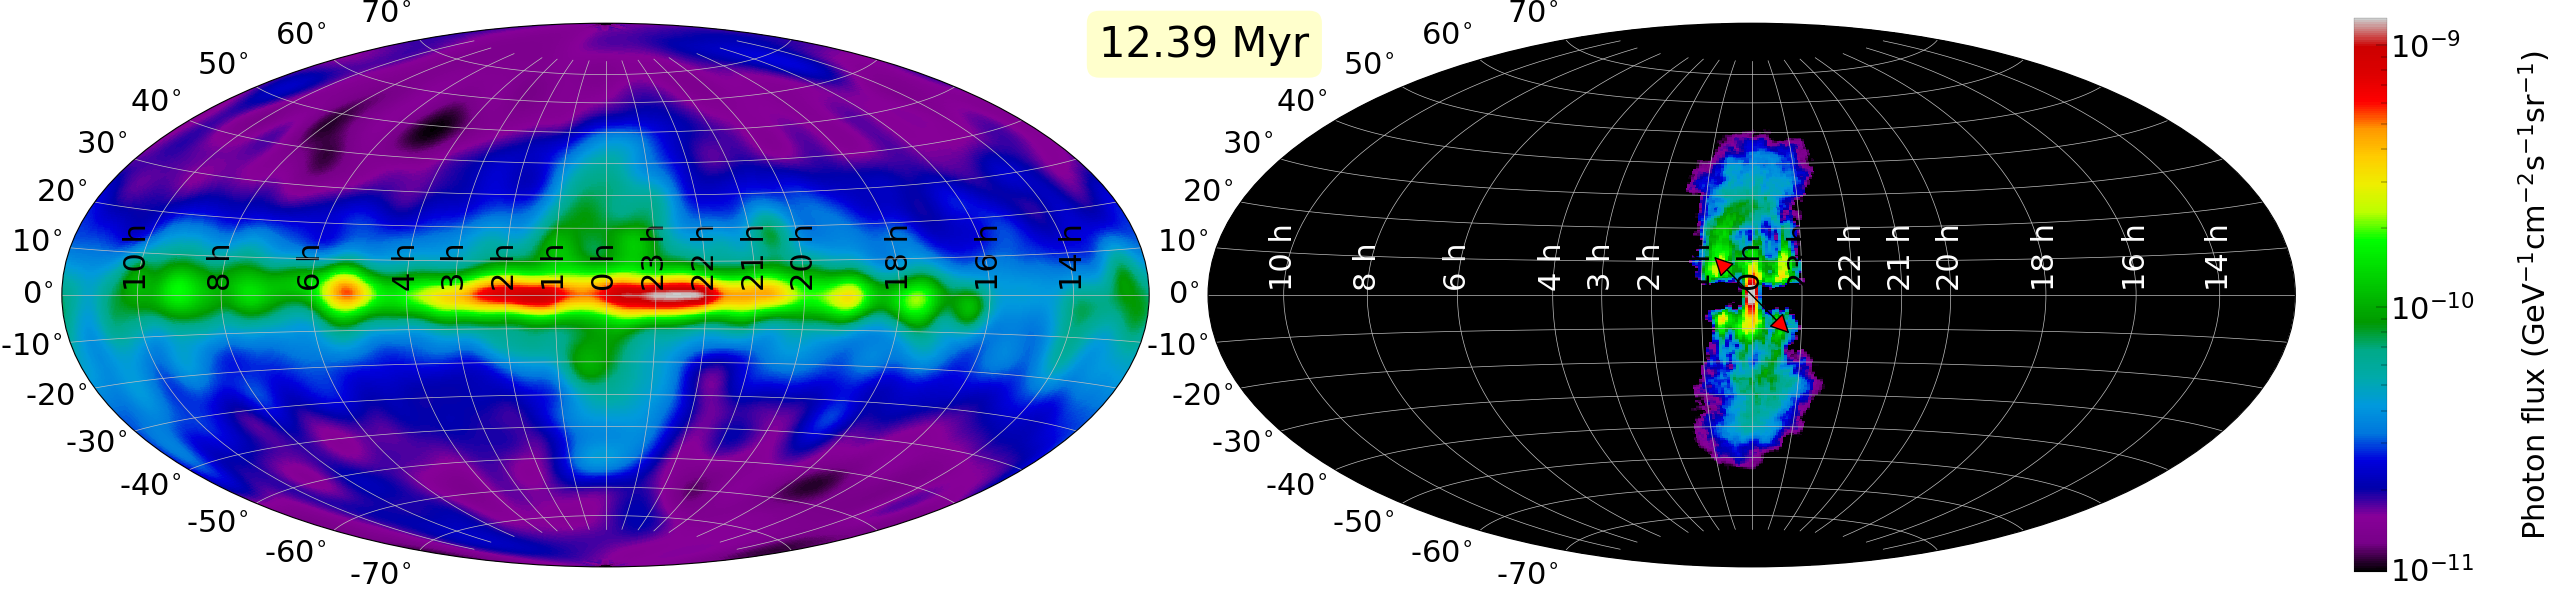
\includegraphics[width=\linewidth]{figures/fig__GammaRay_100e9_1e6_angle_000.png}
  \caption{The observed (left; \citealt{Selig2015}) and simulated (right) photon flux\
           in the energy bin $76.8-153.6$ GeV.\
           Note that the left panel is the\
           photon flux of the diffuse component reconstructed by the D$^3$PO\
           algorithm \citep{Selig2015} that analyzes\
           the photon data from the \textit{Fermi} Large Area Telescope \citep{Atwood2009}\
           and removes the contribution from point-like component.
           The red arrow at the center of the right\
           panel depicts the direction of the bipolar jet, constantly ejecting at an angle of $45^{\circ}$\
           to the disc normal in 1.2 Myr.
  }
  \label{fig__gammaRay-map}
\end{figure*}



  \begin{figure}
    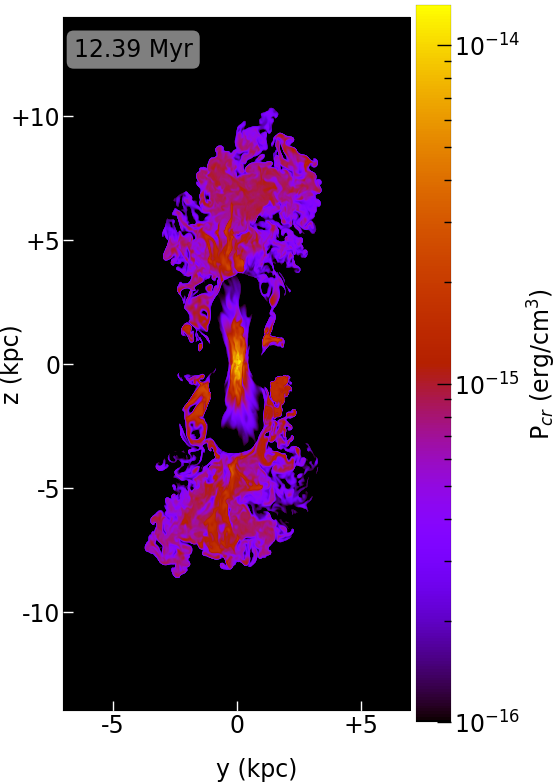
\includegraphics[width=\columnwidth]{figures/fig__jetI5+ismSeed3-45deg-CR.png}
    \caption{
     The CR pressure slice passing through the jet source at 12.39 Myr.\
     Comparison between\
     gas pressure (\Cref{fig__jetI5+ismSeed3-45deg}) and cosmic ray pressure\
     shows that
     the CR pressure\
     is around 5$\times10^{-15}$--8$\times10^{-15}$ erg/cm$^{3}$,\
     bringing the pressure ratio of CR to gas is 0.1--0.2,
     similar to 0.18 at the beginning of the simulation.
     We therefore stress that\
     ignoring the contribution of CR pressure gradient to the momentum of the gas\
     in \Cref{governing-eq} is reasonable.
     }
    \label{fig__jetI5+ismSeed3-45deg-CR}
  \end{figure}



%\subsubsection{Hadronic process}
%In the hadronic model, CRp undergo hadronic collisions with thermal gas protons\
%and produce $\gamma$-ray via pion decay. The volume emissivity of the emission can be written as
%\begin{equation}
%   \epsilon \propto U_{\text{CRp}}n_{p}\sigma_{p}\kappa_{pp}.
%\end{equation}
%
%\begin{equation}
%  \frac{dE}{dtd\epsilon_{1}dV} =\
%   cn_{H}pC\left(\frac{\epsilon_{1}}{m_{\text{p}}c^2}\right)^{-p}\
%   \int_{0}^{1}\sigma(\epsilon_{\text{p}}) F(x,\epsilon_{\text{p}}) x^{p}dx.
%\end{equation}
%
%\begin{equation}
%\sigma(\epsilon_{\text{p}})=34.3+1.88L+0.25L^{2}\left[1-\frac{E_{\text{threshold}}}{E_{\text{p}}}\right]^{4} \text{ mb}.
%\end{equation}
%
%\begin{equation}
%F(x,\epsilon_{\text{p}})=B\frac{d}{dx}\left[\ln(x)\left(\frac{1-x^{\beta}}{1+kx^{\beta}\left(1-x^{\beta}\right)}\right)^4\right],
%\end{equation}
%
%
%where
%$x=\epsilon_{1}/\epsilon_{\text{p}}$, $B=1.30+0.14L+0.011L^2$, $\beta=\left(1.79+0.11L+0.008L^{2}\right)^{-1}$,\
%$\left(0.801+0.049L+0.014L^{2}\right)^{-1}$, $L=\ln(\epsilon_{\text{p}}/1 \text{ TeV})$.



\section{Conclusions}
\label{Conclusions}
In this work, we introduce a thin, dense disk composed of clumpy ISM\
to divert the oblique jets at an angle $45^{\circ}$\
to the disk normal in the past energetic event of the central SMBH.


Also, We investigate the properties of the Galactic bubbles and the microwave\
haze using 3D special relativistic hydrodynamic simulations of CR injection from\
the SMBH assuming the leptonic model.


Our findings are as follows.

\begin{itemize}

\item The Galactic bubbles are nearly symmetric about the Galactic plane albeit\
      the bipolar jets are at an angle $45^{\circ}$\
      with respect to the disc normal.\
      The broad agreement between simulated and observed multiwavelength features\
      provides supporting evidence for the oblique jet scenario, and also\
      releases the caveat given by earlier simulation-based studies:\
      the jets shall be vertical to the disc normal.
\item The randomness of clumpy disk has a insignificant impact on the overall dynamic of the Galactic bubbles.\
      The development of the reverse shocks (the innermost bubbles) are always associated with the dense disc,\
      without the disc, the outermost bubbles and the turbulent plasma will be oblique,\
      indicating the dense disc is crucial for\
      the symmetry of the Galactic bubbles and for the innermost bubbles formation.
\item The edge of the eROSITA bubbles is a forward shock,\
      originally driven by oblique bipolar jets emanating from the GC 12.39 million years ago,\
      and significantly stretched by the stratified atmosphere afterwards.\
      The simulated eROSITA bubbles are not as limb-brightened as the observation.\
      A possibility to enhance the X-ray emission is to include shock-accelerated CRs near the shock,\
      in which CRs could increase the compressibility of the fluid,\
      resulting in the enhanced thermal Bremsstrahlung emissivity that is proportional to density.
\item Followed by the forward shock is a tangling contact discontinuity,\
      which we interpret as the edge of the \textit{Fermi} bubbles.\
      The nature of the \textit{Fermi} bubbles is essentially a turbulent and high-temperature ($\sim2$ keV)\
      plasma in pressure balance with the external medium. Associated with the Galactic magnetic field\
      will lead to the stochastic acceleration of CRe, and probably balanced with the IC and synchrotron cooling.\
      We will investigate the competition between stochastic acceleration and radiative cooling in a future work.
\item According to the microwave and leptonic gamma-ray spectra, the best-fitting\
      CRe power-law index is found to be 2.4.
\item The same leptotonic CRe can simultaneously\
      account for the \textit{Fermi} bubbles and haze emission suggested that\
      they are physically related around the GC,\
      and that the magnetic fields within the bubbles are close to the exponentially distributed\
      Galactic magnetic field.
\end{itemize}



\section{Acknowledgements}
The authors thank Mateusz Ruszkowski and Ellen G. Zweibel for insightful comments.\
We thank Peter Predehl for providing the range of observed X-ray intensity in \Cref{fig__xray_0.8keV_angle_000}.\
A part of the simulations are performed and analyzed using computing resources\
operated by the National Center for High-Performance Computing (NCHC).
HYKY acknowledges support from\
Yushan Scholar Program of the Ministry of Education of Taiwan\
and\
Ministry of Science and Technology of Taiwan (MOST 109-2112-M-007-037-MY3).
HS acknowledges\
funding support from the Jade Mountain Young Scholar Award No. NTU-109V0201,\
sponsored by the Ministry of Education, Taiwan.\
This research is partially supported by the Ministry of Science and\
Technology of Taiwan (MOST) under grants MOST 107-2119-M-002-036-MY3\
and MOST 108-2112-M-002-023-MY3, and the NTU\
Core Consortium project under grants NTU-CC-108L893401 and\
NTU-CC-108L893402.

\section*{Data Availability}
The data underlying this article are available in the article and in its online supplementary material.


%%%%%%%%%%%%%%%%%%%% REFERENCES %%%%%%%%%%%%%%%%%%
\bibliographystyle{mnras}
\bibliography{paper} % if your bibtex file is called example.bib

%%%%%%%%%%%%%%%%% APPENDICES %%%%%%%%%%%%%%%%%%%%%

%\appendix
% https://heasarc.gsfc.nasa.gov/docs/objects/heapow/archive/normal_galaxies/fermibubbles_erosita.html

%Jet_SrcVel 0.6
%Jet_SrcDens 1e-26
%Jet_SrcTemp 2e10
%Jet_SrcPres => 1.6e-8

\end{document}
